\documentclass[10pt, a4paper, twocolumn]{article}
\usepackage{lipsum}
\usepackage[brazilian]{babel}
\usepackage{fancyhdr}
\usepackage{geometry}
\usepackage{graphicx}
\usepackage[T1]{fontenc}
\usepackage{uarial}
\usepackage{indentfirst}
\usepackage[font=small]{caption}
\usepackage{xcolor}
\usepackage{dblfloatfix}
\usepackage{biblatex}

\addbibresource{refs_ciicusp.bib}


\renewcommand{\familydefault}{\sfdefault}
\geometry{a4paper, left=2.6cm, right=2.6cm, bottom=4.2cm, headheight=1.35cm, top=3.4cm}
\setlength{\columnsep}{0.8cm}
\pagestyle{fancy}
\fancyhf{} 
\lhead{
\includegraphics[width=1.6cm]{figures/siicusp.png}}
\renewcommand{\headrulewidth}{0pt}



\begin{document}

\twocolumn[%
  \begin{center}
    {\bf\fontsize{13}{16}\selectfont CLASSIFICAÇÃO MORFOLÓGICA DE GALÁXIAS DO S-PLUS USANDO CONJUNTO DE REDES NEURAIS CONVOLUCIONAIS\\[13pt]}

    {\bf\fontsize{13}{16}\selectfont Natanael Magalhães Cardoso\\[13pt]}

    {\bf\fontsize{13}{16}\selectfont Profa. Cláudia Mendes de Oliveira\\[13pt]}

    {\fontsize{13}{16}\selectfont Instituto de Astronomia, Geofísica e Ciências Atmosféricas, USP -- SP\\[13pt]}

    {\fontsize{10}{12}\selectfont nauxmac@gmail.com}

    \vspace{39pt}
  \end{center}
]


\begin{center}
  \bf\fontsize{13}{15.6}\selectfont Objetivos
\end{center}

A classificação morfológica é a catalogação de galáxias de acordo com a sua aparência visual e a classificação está ligada com as propriedades físicas da galáxia. Uma classificação morfológica feita através de inspeção visual está sujeita a um viés causado pela subjetividade da observação humana. Por isso, a classificação sistemática, objetiva e facilmente reproduzível de galáxias vem ganhando importância desde quando o astrônomo Edwin Hubble criou seu famoso método de classificação \cite{hubble1926}. Neste trabalho, nós combinamos classificações visuais acuradas do projeto GalaxyZoo\footnote{http://galaxyzoo.org} com métodos de \emph{Deep Learning}. O objetivo é encontrar uma técnica automática e eficiente que consiga simular a classificação visual humana a partir da análise de imagens do DR1 do Southern Photometric Local Universe Survey (S-PLUS) \cite{oliveira2019} e publicar um catálogo com galáxias ainda não classificadas. Para isto, um modelo \emph{Deep Learning} foi desenvolvido através de um conjunto de quatro redes neurais convolucionais usando a técnica \emph{Stacking Ensemble} \cite{Wolpert1992}.

\begin{center}
  \bf\fontsize{13}{15.6}\selectfont Métodos e Procedimentos
\end{center}

\begin{figure*}[!h]
  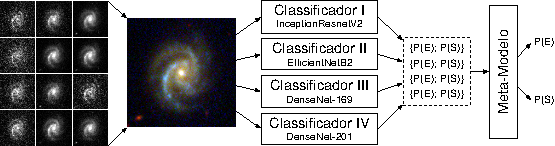
\includegraphics[width=\textwidth]{figures/arch_pt.pdf}
  \caption{Diagrama da arquitetura. Da esquerda para a direita, as 12 imagens de cada banda são agrupadas em uma única imagem RGB, que é a entrada dos classificadores indidviduais. Estes classificadores têm a função de extrair características visuais da imagem e retornar a probabilidade de ser elíptica ou espiral. O meta-modelo tem a função de combinar as predições dos classificadores em uma única predição final mais robusta.}
  \label{fig:arch}
\end{figure*}

O modelo proposto classifica a morfologia das galáxias a partir de suas imagens. As imagens de cada uma das 12 bandas (detalhes sobre cada banda na Tabela 1 de \cite{oliveira2019}) foram obtidas a partir do banco de dados do projeto S-PLUS\footnote{http://splus.cloud}, agrupadas em 3 bandas e convertidas para o espaço de cor RGB. Esta etapa de redução permite usar informações dos 12 filtros do telescópio em imagens com apenas 3 bandas, causando redução no tempo de treino dos modelos. Como a técnica proposta consiste em um treinamento supervisionado, além dos dados a serem classificados, também são necessárias as classificações por humanos do GalaxyZoo para que o algorítmo consiga relacionar os padrões entre as imagens e suas respectivas classes. Foram criados os conjuntos de treinamento, validação e teste, com aproximadamente 30\% de galáxias elípticas e 70\% de galáxias espirais. Técnicas como reamostragem aleatória e ponderamento das classes foram usadas para tratar o desbalanceamento.  Um outro conjunto, denominado \emph{blind}, foi criado com galáxias ainda não classificadas pelo GalaxyZoo e que serão classificadas pelo modelo. Todos estes conjuntos possuem distribuição de \emph{redshift} e magnitude similares.

Para treinar os classificadores, foram usadas redes neurais convolucionais com os pesos inicializados a partir de um pré-treinamento na ImageNet\footnote{http://image-net.org}. O pré-processamento dos dados, o ajuste dos hiper-parâmetros e o treinamento foi feito para cada classificador independentemente. Dos modelos treinados, os que obtiveram melhor performance de classificação são baseados nas arquiteturas InceptionResNetV2, EfficientNetB2, DenseNet-169 e DenseNet-201. Para aproveitar o potencial destes quatro classificadores, um outro modelo (denominado meta-modelo) foi treinado para receber as predições de cada classificador e retornar uma única predição. Formando, assim, um conjunto (\emph{Ensemble}) de classificadores. Este procedimento é resumido no diagrama da Figura \ref{fig:arch}.

% Aquisição dos dados, Divisão dos conjuntos de dados, (Comparação entre os conjuntos), Imagens RGB,

% {Conjunto de dados desbalanceado}, ImageNet (pretreinadas), Aumento de Dados, VGG, IV4, EN, DN, Ensemble, Modelagem dos Classificadores e Ensemble


\begin{center}
  \bf\fontsize{13}{15.6}\selectfont Resultados
\end{center}

\begin{figure}[!b]
  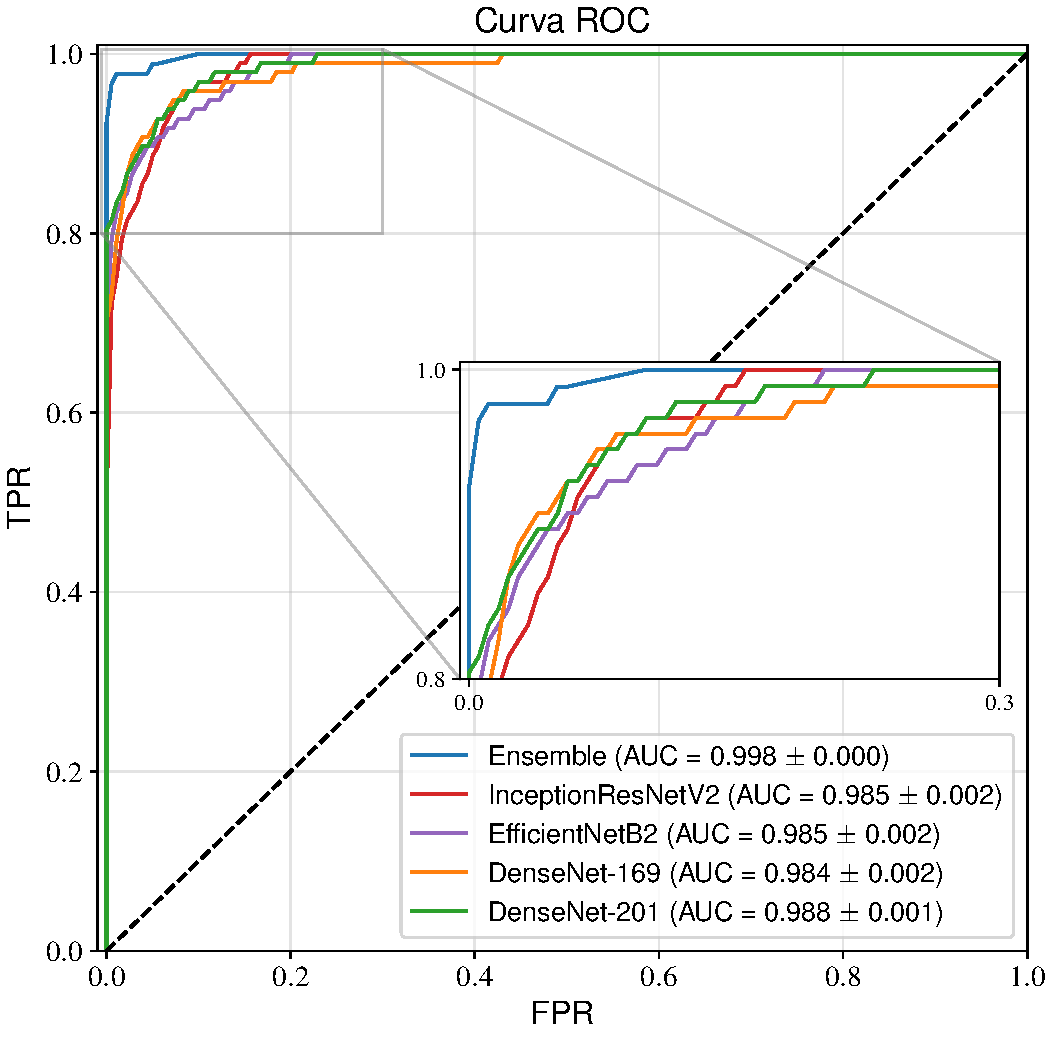
\includegraphics[width=\linewidth]{figures/roc_mn170_pt.pdf}
  \caption{Curva ROC para cada classificador e para o \emph{Ensemble}. Cada curva representa a mediana de 60 medições, a área abaixo da curva (AUC) e seu desvio padrão estão na legenda de cada curva.}
  \label{fig:roc}
\end{figure}

Uma forma de avaliar o modelo quantitativamente é a partir da Curva Característica de Operação do Receptor (ROC) no conjunto de teste, como mostra a Figura \ref{fig:roc}. A partir deste gráfico é possível tirar conclusões sobre o potencial de classificação do modelo. A área abaixo da curva, cujo valor máximo é 1, indica a propabilidade de classificação correta pelo modelo. Além disso, quanto mais rápido a curva chega ao topo, maior é o grau de separabilidade do modelo, ou seja, maior a capacidade do modelo de distinguir entre as classes. Como esperado, o Ensemble (curva azul), que é a união dos quatro classificadores, supera a performance dos classificadores individualmente, atingindo uma AUC de 0.998.


\begin{center}
  \bf\fontsize{13}{15.6}\selectfont Conclusões
\end{center}

A partir deste projeto foram obtidos um modelo de \emph{Deep Learning} completamente desenvolvido e operante com alto potencial de classificação morfológica entre galáxias elípticas e espirais a partir de imagens do S-PLUS, além de um catálogo com classificações automatizadas de 2536 galáxias com magnitude menor que 17 sem classificações no GalaxyZoo, ambos publicamente disponíveis\footnote{http://natanael.net}. Além disso, um artigo científico sobre este projeto encontra-se em etapa final de escrita.



\begin{center}
  \bf\fontsize{13}{15.6}\selectfont Referências Bibliográficas
\end{center}

\printbibliography[heading=none]


\end{document}